\section{Auswertung}

\subsection{Strahlungsbelastung}

Da für das Experiment radioaktive Präparate benutzt werden, scheint eine
Abschätzung der maximalen, persönlichen Belastung sinnvoll.

Folgende Annahmen wurden getroffen:
\begin{itemize}
  \item Die betreffende Person wiegt $m = \SI{80}{\kilo\gram}$.
  \item Die Einwirkdauer beträgt jeweils $s = \SI{12}{\hour}$.
  \item Die Aktivität $A$ aller 3 Präparate übersteigt jeweils nicht
        \SI{4e5}{\becquerel}.
  \item Die Halbzeit $t$ aller 3 Präparate wird mit dem maximalen Wert, 30 Jahren,
        abgeschätzt.
  \item Seit der Vermessung der Präparate sind aufgerundet $u = $ 3 Jahre vergangen.
  \item \SI{100}{\percent} der Strahlung wird aufgenommen.
  \item Der Strahlungsgewichtungsfaktor für γ-Strahlung beträgt 1.
  \item Die γ-Quanten haben eine maximale Energie von
        $E = \SI{0.7}{\mega\eV} = \SI{1.12e-13}{\joule}$
  \item Es gibt $n = 3$ Proben.
\end{itemize}
Damit berechnet sich die radioaktive Belastung zu
\begin{equation}
  s \left(\frac{1}{2}\right)^{u/t} n E A / m = \SI{0.07}{\milli\sievert}
\end{equation}
und macht somit bei einer durchschnittlichen Strahlungsbelastung in Deutschland von
\SI{4.3}{\milli\sievert} pro Jahr rund \SI{2}{\percent} aus.

\subsection{Signalbetrachtung}
In unserem Experiment wurde ein Szintillationsdetektor, an den ein
Photomultiplier angeschlossen war, verwendet, um ankommende Photonen in ein
messbares elektrisches Signal umzuwandeln. Dieses Signal wurde anschließend
durch einen Vorverstärker und zusätzlich noch durch einen Hauptverstärker
geleitet. Auch wenn sich in der Nähe des Detektors keine radioaktive Quelle
befand wurden trotzdem Signale gemessen, was hauptsächlich durch das thermisch
bedingtes Rauschen der beteiligten Komponenten verursacht wurde. Diese
Rausch-Signale konnten beobachtet und auf ihre Form hin untersucht werden.

Sowohl das Signal des Vorverstärkers als auch des Hauptverstärkers kann in
\fref{signalform} betrachtet werden.
\begin{figure}[htb]
      \centering
      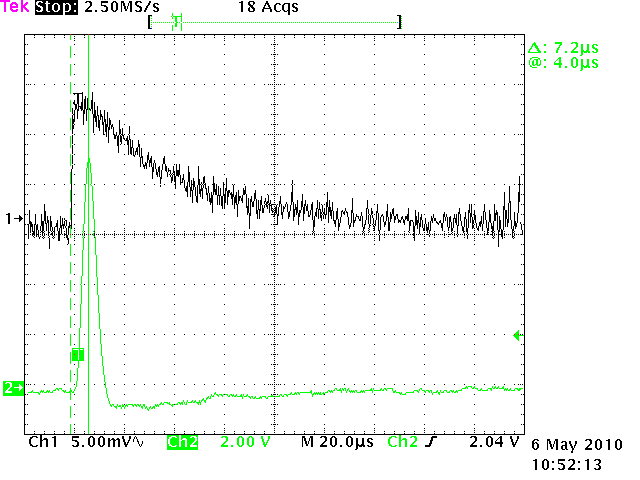
\includegraphics[width=1\columnwidth,keepaspectratio]{signalform}
      \caption{Standbild des Digital-Oszilloskops zur Signalform-Betrachtung}
      \label{fig:signalform}
\end{figure}

Man kann erkennen, dass die schwarze Linie dem Vorverstärkersignal entspricht,
was dadurch deutlich wird, dass die Achseneinteilung (an Channel 1) bei gerade
einmal \si{5}{\milli\volt} pro Kästchen lag, während das noch einmal verstärkte
Hauptverstärkersignal (grüne Linie) bei einer Achseneinteilung von
\si{2}[{\volt} aufgetragen wurde. Offenbar wird das Signal im Hauptverstärker
noch einmal geglättet, denn dessen Signal entspricht einer Gauß-Kurve, wobei im
Gegensatz dazu das Vorverstärkersignal sprungartig ansteigt, dann aber viel
Zeit braucht, um wieder auf das Niveau vor der Messung abzufallen (man kann
grob abschätzen, dass das Vorverstärkersignal ungefähr
$6\cdot20\si{\micro\second} = 120\si{\micro\second}$ für den Abfall benötigt,
wohingegen das Hauptverstärkersignal nur etwa 10\si{\micro\second} braucht.)

\subsection{Latenzzeit der Messtechnik}

\begin{figure}[htb]
      \centering
      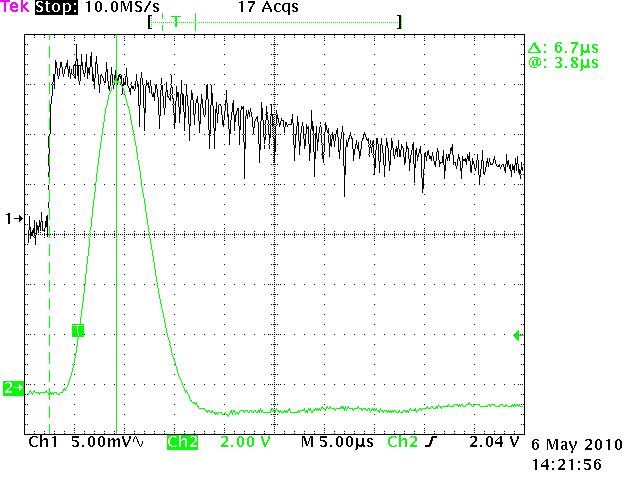
\includegraphics[width=1\columnwidth,keepaspectratio]{messverzoegerung}
      \caption{Standbild des Digital-Oszilloskops zur Messung der Latenzzeit}
      \label{fig:latenz}
\end{figure}

Durch die Verwendung des Hauptverstärkers kann das Signal mit höherer Präzision
gemessen werden, jedoch muss man dafür eine zeitliche Verzögerung $Δt$ in Kauf
nehmen. Um jene zu bestimmen, wird der Trigger des Oszilloskops auf den
Vorverstärker gestellt, die Schwellspannung für das Triggern auf einen Wert
hochgeregelt, der nur bei Eintreffen eines Signals erreicht wird und nicht
durch die permanente Fluktuation, und dann wurde das Bild manuell angehalten, so
dass im Ergebnis ein Standbild wie in \fref{latenz} exportiert werden kann.
Hierfür haben wir die Zeitskala kleiner eingestellt, um bessere Messungen
vornehmen zu können. Das Rädchen, mit dem die Ablesehilfe verschoben werden
konnte, ließ sich in der gewählten Einstellung in
0,1\si{\micro\second}-Schritten verstellen. Damit ist jeder einzelne Messwert
mit diesem zufälligen Fehler behaftet. Da in diesen Schritten eindeutig
erkennbar war, bei welcher Schieber-Position das Maximum der
Hauptverstärkerkurve sowie der Sprung in der Vorverstärkerkurve zu finden ist,
tragen diese ``Ableseungenauigkeiten'' kaum zum zufälligen Fehler bei und
werden vernachlässigt. Systematische Fehler könnten aufgetreten sein (z.B.
durch eine konstante Verzögerung zwischen Channel 1 und Channel 2), aber da wir
dazu keine Aussage treffen können, betrachten wir auch solche Fehler nicht
weiter. Die somit resultierenden Ergebnisse können in \tref{latenzmesswerte}
betrachtet werden.
\begin{table}[htbp]
\centering
% \setlength{\tabcolsep}{14pt}
\begin{tabular*}{\columnwidth}{%
S[tabformat=1.1]%
S[tabformat=1.1]%
S[tabformat=1.1]%
S[tabformat=1.1]%
S[tabformat=1.1]%
S[tabformat=1.1]%
S[tabformat=1.1]%
S[tabformat=1.1]%
}
\toprule
{$x_1$} & {$x_2$} & {$x_3$} & {$x_4$} & {$x_5$} & {$x_6$} & {$\bar x$} & {$Δx$}\\
\midrule
6.7 & 6,8 & 6,5 & 6.8 & 6.8 & 6.6 & 6.7 & 0,2 \\
\bottomrule
\end{tabular*}
\label{tab:latenzmesswerte}
\caption{Messwerte der Latenzzeit}
\end{table}
Die Latenzzeit beträgt somit
\begin{equation}
  Δt = \SI{6.7(2)}{\micro\second}
\end{equation}
. Der angegeben Fehler ist dabei die
Standardabweichung $\sigma_s$, und das Vertrauensintervall beträgt 0,06. Die
Standardabweichung wurde nach der üblichen Methode (s. \cite[S.10]{barlow})
berechnet: 
\begin{equation}
  \sigma_s = \sqrt{\frac{1}{N}\sum_{i=1}^N(\overline{x}-x_i)^2}
\end{equation}
In unserem Fall war $N=6$.

Da die Öffnungszeit jedoch vom Computer vollautomatisch
gemessen wird, ist eine Latenzzeit in diesen Versuch unerheblich.

\subsection{Untergrundmessung}

\subsection{Eichung}

\subsection{Bestimmung des totalen Compton-Wirkungsquerschnitts}
Das Ziel der folgenden Betrachtungen ist die Berechnung des totalen
Wirkungsquerschitts für Compton-Streuung. Wir betrachten dafür die Tatsache,
dass Teilchen, die mit dem Festkörper, also dem Aluminiumblock, gewechselwirkt
haben, anschließend in erster Näherung ihre Richtung verändern und somit vom
Detektor nicht mehr registriert werden können. Diese Annahme ist sicherlich
nicht vollständig korrekt und wird daher später noch diskutiert. Die
Messgrößen, die sich für die Betrachtung anbieten, sind demnach die Anzahl der
registrierten Photonen ohne ein Aluminium-Hindernis $N_0$ sowie die Zahl der
Photonen $N'$ mit einem Aluminium-Block zwischen Quelle und Detektor. Um daraus
den Wirkungsquerschitt zu berechnen, verwenden wir die aus der Vorlesung
``Einführung in die Kern- und Teilchenphysik'' bei Hr. Prof. Lohse bekannte
Beziehung
\begin{eqnarray}
  N'(x) &=& N_0 \mathrm e^{-\sigma \rho_T x}\\
\rightarrow \sigma &=& \frac{1}{\rho_T x}\ln\left(\frac{N_0}{N'(x)}\right)
\end{eqnarray}
In unserem Fall ist die Dicke des Aluminiumblocks mit $x = d =
\si{5}{\centi\meter}$ bekannt und konstant, sodass aus der obigen Formel
resultiert:
\begin{equation}
  \sigma = \frac{1}{\rho_T d}\ln\left(\frac{N_0}{N'}\right)
\end{equation}
Es bleibt zu klären, welchen Wert die Dichte der Streuzentren $\rho_T$, in
diesem Fall die Elektonendichte für Aluminium, besitzt. Dabei kann man
auf die bekannte Massendichte $\rho$ sowie auf die molare Masse $A$
zurückgreifen:
\begin{equation}
  \rho_T = \frac{N_A}{A}\cdot Z\rho
\end{equation}
Hier ist $N_A$ die Avogadro-Konstante, die \cite{pdb} entnommen wurde, die
drei anderen Größen wurden \cite[Tab.2]{script} entnommen. Die Zahl der
Elektronen pro Volumeneinheit lautet somit:
\begin{equation}
  \rho_T = 7,83\cdot 10^{23} \cdot \frac{1}{\si{\centi\meter^3}}
\end{equation}

Nachdem wir diesen Wert bestimmt haben, können wir nun die verbliebenen
Unbekannten in der Wirkungsquerschittsformel betrachten. Da wäre zum einen die
Anzahl der ungehindert passierten Photonen $N_0$. Diese Zahl ergibt sich aus
der Fläche unter dem Photopeak. Um diese Fläche bestimmen zu können, wurde im
letzten Abschnitt bereits ein Programm erstellt, das von den normierten
Messdaten, die bei Vorhandensein einer Quelle gemessen wurden, ein normiertes
Untergrundspektrum abzieht, sodass bis auf eine gewisse Fluktuation nur noch
uns interessierendes physikalisches Signal vorhanden ist. Dieses
Photopeak-Signal wurde in einem gewissen Bereich mit einer Gauß-Verteilung
gefittet. Da man nun eine Funktion gegeben hat, deren Fläche man (zumindest
numerisch) berechnen kann. Weil aber unsere Grenzen, in denen gefittet
wird, willkürlich festgelegt sind, sollte man versuchen, die Integration
möglichst unabhängig von dieser Wahl zu machen. Daher berechnen wir die
Photopeakfläche durch eine Integration von $-\infty$ bis $+\infty$. Bei
einer Gaußkurve ist das Ergebnis einer Integration in diesen Grenzen bekannt,
und somit brauchen wir uns um die Integration selbst keine Gedanken mehr zu
machen und müssen nur noch die Fit-Parameter einsetzen.

Allgemein sieht eine Gauß-Funktion folgerndermaßen aus:
\begin{equation}
  N(c) = N_{max}\mathrm e^{-\frac{(c-\mu)^2}{s^2}}
\end{equation}
Dabei steht die Variable $c$ in diesem Fall für den Channel, während die
anderen Größen, also $N_{max}$ für den Maximalwert der Verteilung, $\mu$ für den
Mittelwert und $s$ als Maß für die Breite der Gaußfunktion, die Fitparameter
sind. Für den $^{137}$Cs-Photopeak ohne Aluminiumblock ergeben sich bei einer
solchen Fitfunktion die folgenden Werte:
\begin{eqnarray}
N_{max} &=& 0,13\\		%fehlerbetrachtung!!!
\mu &=& 994\\
s &=& 65
\end{eqnarray}

Somit kann man auch problemlos die Fläche $N_0$ unter dieser Kurve
angeben, was gleich der uns interessierenden Anzahl der ungestört eintreffenden
Photonen ist:
\begin{eqnarray}
N_0 &=& \int\limits_{-\infty}^{+\infty}N(c)dc\\
&=& N_{max}\sqrt{\pi}\cdot s\\
\nonumber &=& 0123456789
\end{eqnarray}
Um die Effizienz der Detektion muss man sich keine Gedanken machen, da uns am
Ende ohnehin nur das Verhältnis der Teilchenzahlen interessiert.

Wenn man das gleiche Verfahren auf das Signal, das mit dem Aluminiumblock als
Hindernis aufgenommen wurde, anwendet, so ergeben sich die folgenden Daten:
\begin{eqnarray}
N_{max} &=& \\
\mu &=& \\
s &=& 
\end{eqnarray}
Damit ergibt sich als Fläche unter der Kurve $N'$:
\begin{equation}
N' = 
\end{equation}

Damit schließlich lässt sich der Wirkungsquerschitt $\sigma$ aurechnen:
\begin{eqnarray}
\sigma &=& \frac{1}{\rho_T d}\ln\left(\frac{N_0}{N'}\right)\\
\nonumber &=& 
\end{eqnarray}

% kommentare,...
% evtl nächster absatz

\subsection{Korrektur des Wirkungsquerschnitts}
Abschließend ist der berechnete Wirkungsquerschitt um einen gewissen Betrag zu
korrigieren, da bisher nur der Photonen betrachtet wurden, die entweder den
Aluminiumblock ungehindert passiert haben oder aber von diesem gestreut wurden
und daher nicht detektiert werden konnten. Allerdings haben wir dabei bisher
nicht berücksichtigt, dass es auch möglich ist, dass manche Photonen
Comptonstreuung durchführen und trotzdem kaum ihre ursprüngliche Flugbahn
ändern, sodass sie immernoch gemessen werden können. Diese Korrektur soll im
Folgenden näherungsweise durchgeführt werden.

Wir gehen davon aus, dass der Photonenstrahl perfekt kollimiert ist, senkrecht
zur Detektorfläche fliegt und auf der Höhe des Mittelpunkts der Detektorfläche
in den Aluminiumblock eintritt. Weiterhin gehen wir davon aus, dass die
Comptonstreuung erst am Ende des Al-Blocks stattfindet. Dann kann leicht der vom
Detektor eingenommene Raumwinkel $\Omega_{\mathrm{Det}}$ berechnet werden. Als
Resultat einer kurzen Rechnung lautet dann:
\begin{equation}
\Omega_{\mathrm{Det}} = 
\end{equation}
Im letzten Abschnitt aber haben wir eigentlich den Wirkungsquerschnitt dafür
berechnet, dass Photonen so gestreut werden, dass sie anschließend nicht mehr
detektierbar sind. Um also diese Näherung nicht treffen zu müssen, berechnen wir
nun aus den gegebenen Größen die wahre Anzahl $N'_{\mathrm{korr}}$ der Photonen,
die den Aluminiumblock wirklich ohne Wechselwirkung passiert haben. Nach einer
etwas längeren Rechnung erhalten wir als Ergebnis:
\begin{eqnarray}
N'_{\mathrm{korr}} &=& \frac{N_{\mathrm{mit Al}}-cN_0}{1-c}\\
c &=& \frac{\Omega_{\mathrm{Det}}}{4\pi}\\
\rightarrow N'_{\mathrm{korr}} &=& 
\end{eqnarray}
Da nun die korrigierte Zahl der Teilchen bekannt ist, die ohne Wechselwirkung
zum Detektor gelangten, kann man leicht den korrigierten
Compton-Wirkungsquerschnitt $\sigma_{\mathrm{korr}}$ berechnen:
\begin{eqnarray}
\sigma_{\mathrm{korr}} &=& \frac{1}{\rho_T
d}\ln\left(\frac{N_0}{N'_{\mathrm{korr}}}\right)\\
&=& 
\end{eqnarray}